\documentclass{beamer}
\usepackage{graphicx}

\setbeamertemplate{footline}[frame number]

\begin{document}
\title{Array-Based Topological Mesh Representation
 Supporting General Modification}
\author{Dan Ibanez}

\frame{\titlepage}

\frame{\frametitle{Overview}
We present a mesh data structure with novel properties:
\begin{itemize}
\item composed of several large arrays
\item addition and removal are $O(1)$ operations
\item supports mixed element types
\item stores arbitrary associated data
\item uses 4x less memory than object-based versions
\item efficiently supports parallel meshes
\end{itemize}
}

\frame{\frametitle{Basic Mesh Data Structure}
The simplest mesh data structure is an element to
node connectivity array.

Given an integer element id, returns the integer
node ids of that element.

Sufficient for element integration, element
stiffness matrix assembly, etc.

\vskip 20pt

\begin{center}
\includegraphics[width=0.4\textwidth]{ibanez_cse15-1.png}
\hspace{30pt}
\includegraphics[width=0.4\textwidth]{ibanez_cse15-2.png}
\end{center}
}

\frame{\frametitle{Adjacency Graph}
Element to node connectivity forms a bipartite graph
where all elements of the same topological type
have the same degree.

In the example, both elements are quadrilaterals.

\begin{center}
\includegraphics[width=0.6\textwidth]{ibanez_cse15-3.png}
\end{center}
}

\frame{\frametitle{Upward Adjacency}
The inverse of element-node connectivity, i.e.
which elements are adjacent to a node.

This is harder, because the degrees are not the same.

Object-based structures may store many small arrays.

\begin{center}
\includegraphics[width=0.6\textwidth]{ibanez_cse15-4.png}
\end{center}

Required during any kind of mesh modification, including
element load balancing.
}

\frame{\frametitle{Linked Upward Adjacency}
A more compact but equivalent format:
The entries of the upward array are arranged
to match the ordering of the downward array, such
that the same graph edge has the same index.

\begin{center}
\includegraphics[width=0.6\textwidth]{ibanez_cse15-6.png}
\end{center}

Element id is now implicit by location, but
entries are non-contiguous and must be linked.
Graph edges from the same graph node are linked together.
}

\frame{\frametitle{Upward Adjacency Arrays}
Since the element id can be derived from the entry's
position, we can use the entries to store list links
instead.
Another array for the nodes points to the head
of the list.

\begin{center}
\includegraphics[width=0.6\textwidth]{ibanez_cse15-7.png}
\end{center}

Array indices are used instead of pointers.
Upward adjacency can still be derived by traversing
these lists-in-arrays.
}

\frame{\frametitle{Mesh Modification}
\begin{itemize}
\item
All mesh modifications are implemented as element
addition and removal.

\item
We have arrays of size $CN$ where $N$ is the
number of entities of one type,
and each $C$ contiguous entries
correspond to the same entity.

\item
We need general array modification algorithms
for adding and removing entries
(or contiguous $C$ entries).

\item
Finally, we control where addition happens, users
just want storage for a new entity.
\end{itemize}
}

\frame{\frametitle{Array Addition}
\begin{itemize}
\item
Common solution is geometric growth with additions to the end.
For example, the C++ std::vector uses this algorithm.
\item
Array has allocated capacity $(c)$ and used size.
When addition is requested and used size equals capacity,
reallocate to capacity $\alpha c$, $\alpha > 1$.
We use $\frac32(c+1)$.
\item
Result is amortized $O(1)$ insertion at the end.
\item
{\bf C}'s \texttt{realloc()} can be more efficient due
to virtual memory page mapping...
\end{itemize}
\begin{center}
\includegraphics[width=0.4\textwidth]{ibanez_cse15-9.png}
\end{center}
}

\frame{\frametitle{Array Removal}
\begin{itemize}
\item
Removal can happen anywhere, leaves a hole.
\item
Trying to fill the hole requires moving another
entry or entries
\item
But changing indices is bad for users, they
need unique consistent identifiers
\item
So, keep the holes and track them
\end{itemize}
}

\frame{\frametitle{Free List}
\begin{itemize}
\item
One array per entity type, tracks holes in other arrays
\item
Holes are linked together in one ``free list".
\item
On removal, new hole is linked to front of list.
\item
On addition, check for holes and, if any, unlink
the first hole from the list and fill it.
\item
Non-holes receive a ``Live" value (-2) to distinguish
from valid linked list values $[-1,\infty)$.
\end{itemize}

\begin{center}
\includegraphics[width=0.6\textwidth]{ibanez_cse15-8.png}
\end{center}
}

\frame{\frametitle{Array Modification Algorithm}
On removal, link new hole into free list.

On addition:
\begin{enumerate}
\item
If there are holes, unlink the first hole
and return its index
\item
If used size equals capacity, reallocate for
bigger capacity
\item
Increment used size, return last index
\end{enumerate}

\vspace{20pt}

\includegraphics[width=0.8\textwidth]{flex.png}

}

\frame{\frametitle{Element-Vertex Structure}

A reduced mesh representation with only elements
and vertices would use the following set of arrays:

\begin{itemize}
\item Vertex free list array
\item Element free list array
\item Element to vertex array
\item Vertex to element lists-in-arrays
\item Simulation field arrays, indexed by vertex id
\end{itemize}

\begin{center}
\end{center}
}

\frame{\frametitle{Memory Analysis}
\begin{itemize}
\item theoretical memory use for reduced tetrahedral mesh
\item static pointers =
$(4+4)n_{tet} + (3)n_{vtx}$
\item with free list =
$(1+4+4)n_{tet} + (1+3)n_{vtx}$
\item estimated ratios
\[n_{vtx} = n_{tet}/6\]
\item with free list, 56 pointers per vertex, ~9.7 pointers per element
\item using 32-bit index ``pointers", ~40 bytes per element
\item with non-topological data added, uses ~50 bytes
per element
\end{itemize}
}

\frame{\frametitle{Memory Use Comparison}
\begin{center}
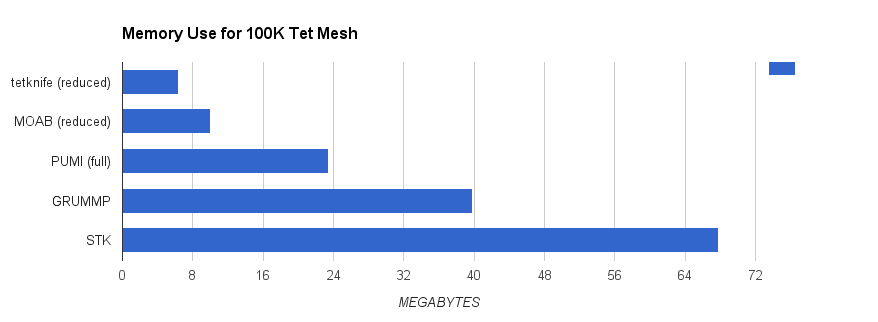
\includegraphics[width=1.0\paperwidth]{memory_comparison.png}
\end{center}
}

\begin{frame}
\frametitle{1.6 Billion Element Mesh Generation}
\begin{center}
\includegraphics[width=0.8\textwidth]{scl_ref_nelem_total.png}
\end{center}
\begin{itemize}
\item start with 100K element mesh on rank 0
\item repeat 14 times ($2^{14} = 16384$)
\begin{itemize}
\item use Cavity Operator to make 2X more elements
\item use global RIB to partition to 2X more cores
\end{itemize}
\end{itemize}
\end{frame}

\begin{frame}
\frametitle{Runtime of Steps}
\begin{center}
\includegraphics[width=0.8\textwidth]{scl_time.png}
\end{center}
\begin{itemize}
\item Total runtime: 288 seconds
\item (without link-time optimization, 884 seconds)
\item Entirely in-memory, no files, one MPI batch job
\end{itemize}
\end{frame}

\begin{frame}
\frametitle{Heap Memory Usage}
\begin{center}
\includegraphics[width=0.8\textwidth]{scl_bal_heap.png}
\end{center}
\begin{itemize}
\item 200K elements max + remote copies + MPI + misc
\end{itemize}
\end{frame}

\begin{frame}
\frametitle{Balance after Cavity Operator}
\begin{center}
\includegraphics[width=0.8\textwidth]{scl_ref_imb.png}
\end{center}
\begin{itemize}
\item RIB does ``perfect" rebalance on this cube
\end{itemize}
\end{frame}

\begin{frame}
\frametitle{Neighbor Counts}
\begin{center}
\includegraphics[width=0.5\textwidth]{scl_ref_neigh.png}
\includegraphics[width=0.5\textwidth]{scl_bal_neigh.png}
\end{center}
\begin{itemize}
\item left is after refinement, right is after balance
\item 26 is theoretical for uniform grid under RIB
\end{itemize}
\end{frame}

\frame{\frametitle{Acknowledgements}
This material is based upon work supported by the
U.S. Department of Energy, Office of Science,
Office of Fusion Energy Sciences and
Office of Advanced Scientific Computing Research under
Award Number DE-SC0006617
(Frameworks, Algorithms, and Scalable Technologies for Mathematics).

\vspace{40pt}

\begin{center}
{\it Thank You... Questions ?}
\end{center}

\vspace{40pt}
}

\end{document}

